
\documentclass[10pt]{article}
\usepackage[utf8]{inputenc}
\usepackage{kotex}
\usepackage{graphicx}
\usepackage{subfigure}
\usepackage{titling}
\setlength{\droptitle}{-2cm}
\usepackage{array}
\usepackage{amssymb}
\usepackage{amsmath}
\usepackage{siunitx} 
\usepackage{enumerate} 
\usepackage{pgfplots}
\usepackage{pgfplotstable}
\usepackage{tikz,pgfplots}
\usepackage{wasysym}
\usepackage{geometry}
\usepackage{authblk}
\usepackage{kotex}
\usepackage{bibunits}
\usepackage{tabularx}
\usepackage{hyperref}
\usepackage{pythonhighlight}

\geometry{
    a4paper,
    total={170mm,257mm},
    left=20mm,
    top=20mm,
}

\title{\textbf{Mathematical Foundation of DNN : HW 12}}
\author{Jeong Min Lee}

\begin{document}
\maketitle

\section*{1}

\begin{figure}[!h]
    \begin{center}
        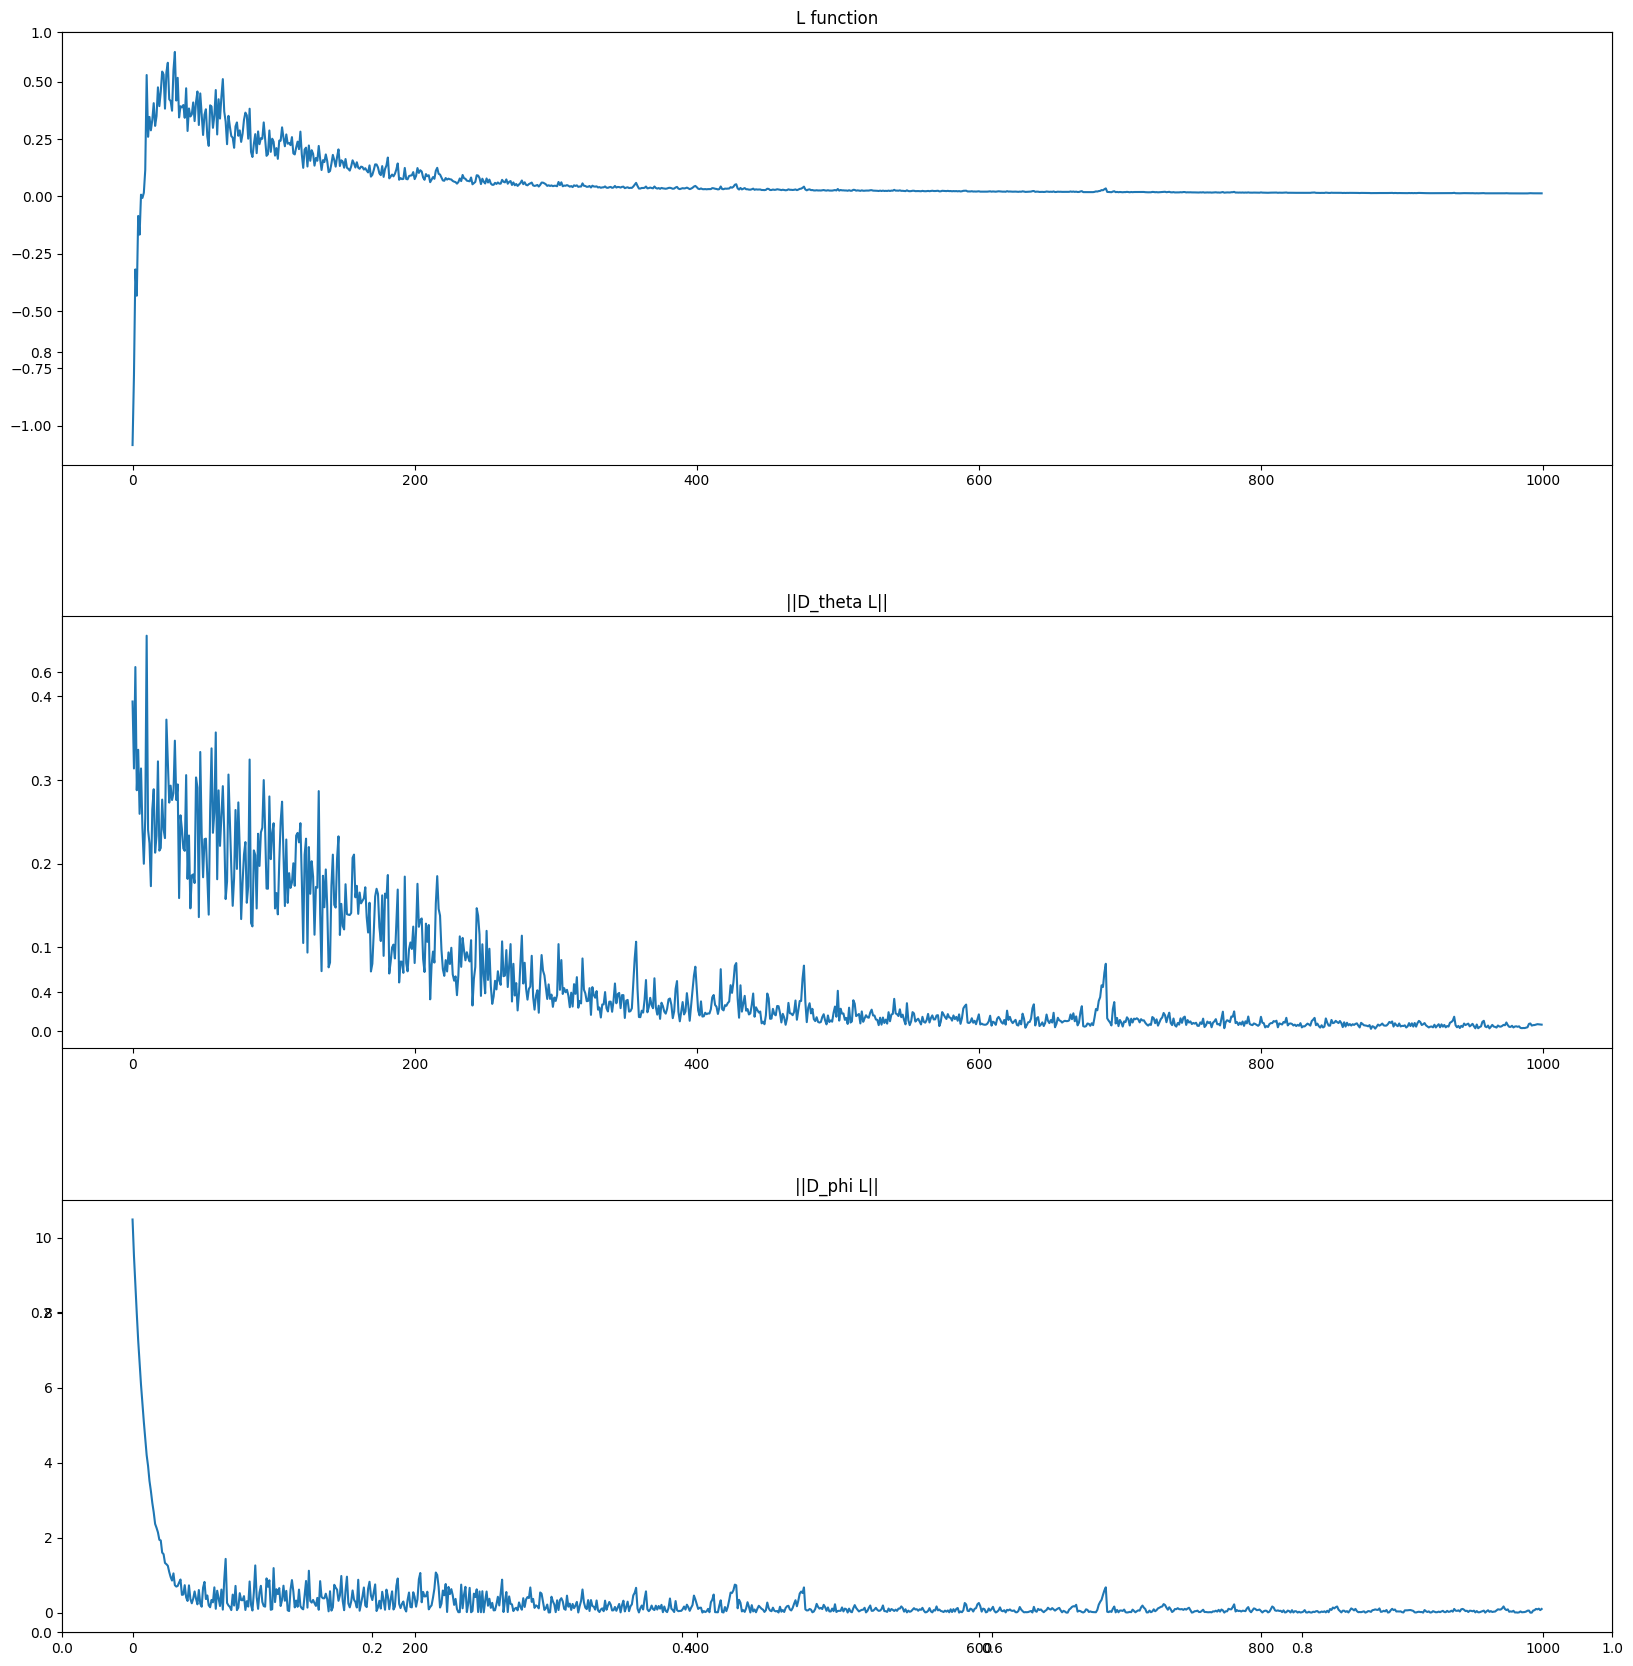
\includegraphics[scale = 0.3]{fig1.png}
        \caption{Loss and its gradient of the model's parameters. }
        \label{fig1}
    \end{center}
\end{figure}
As the Figure \ref{fig1} shows, the loss and its gradient converge to the zero.
This implies that the training of robust logistic model is successful.
Note that the uneven and jittering curve is originated from the nature of SGD.
Please, refer to the jupyter notebook file to see the implementation. 
\section*{2}
First of all, one have to verify that $f(u)$ is convex or not. To confirm it, it is necessary to find second derivative of $f(u)$ and its sign.
\begin{align*}
    {d^2 \over du^2} f(u) = \frac{1}{u} - \frac{1}{u+\lambda} = \frac{\lambda}{u(u+\lambda)}
\end{align*} 

Since the domain of $f(u)$ is $\left\{u\in \mathbb{R} | u \ge 0\right\}$ and the regularization coefficient $\lambda$ is positive, $f^{\prime\prime}(u)>0$.
This implies that $f(u)$ is convex function in its domain.
Then, find the convex conjugate of $f(u)$, $f^*(t)$.
\begin{align*}
    f^*(t) &= \underset{u\in\mathbb{R}}{\sup}\left\{tu - f(u)\right\} \\
    &= \underset{u\in\mathbb{R}}{\sup}\left\{tu - u\log\frac{u}{u+\lambda} - \lambda \log \frac{\lambda}{u + \lambda} - (1+\lambda)\log(1+\lambda) +\lambda \log \lambda\right\}
\end{align*}
To evaluate the $f^*(t)$ or the supremum of $tu-f(u)$, take first derivative of $tu-f(u)$ to find where the supremum is.
\begin{align*}
    &{d\over du} tu-f(u) =  t - f^\prime(u) \\
    &t-\log u + \log(u+\lambda) = 0  \\
    & \therefore u = \frac{\lambda}{e^{-t}-1}
\end{align*}
Thus, \begin{align*}
    f^*(t) &= \frac{t\lambda}{e^{-t}-1} - \frac{\lambda}{e^{-t}-1}\log e^t - \lambda \log(1-e^t) -(1+\lambda)\log(1+\lambda) + \lambda \log \lambda\\
    &=-\lambda \log(1-e^t) -(1+\lambda)\log(1+\lambda) + \lambda \log \lambda
\end{align*}
Recall \begin{equation*}
    D_f(p_{true}||p_\theta) = \underset{T\in\mathcal{T}}{\sup}\left\{\mathbb{E}_{X\sim p_{true}}[T(X)] - \mathbb{E}_{\tilde{X}\sim p_\theta}[f^*(T(\tilde{X}))]\right\}
\end{equation*}

Although the bias term in $f^*(t)$ do affect to the maximum and minimum, it cannot affect to the gradient of the loss function and the optimum without taking the bias term into the consideration is same to that with bias term. This give us the background of deleting the bias term of $f^*(t)$.
Therefore, the $f$-divergence is given as follow.
\begin{equation*}
    D_f(p_{true}||q) = \underset{T\in \mathcal{T}}{\sup}\left\{\mathbb{E}_{X\sim p_{true}}[T(X)] + \lambda \mathbb{E}_{\tilde{X} \sim p_\theta}\left[\log(1-e^{T(\tilde{X})})\right]\right\}
\end{equation*} 
By replacing $T(x) = \log D_{\phi}(x)$, one can observe that the given minmax problem is identical to GAN with non-uniform weights.

\section*{3,4}
To implement the GAN and VAE, I refered to the example code in lecture.
As Figure \ref{fig2},\ref{fig3} depicts, the reconstruction of Swiss roll data is success, noting that the final data distribution is resemble to the that of original one. 
\begin{figure}[!h]
    \begin{center}
        \subfigure[]{
            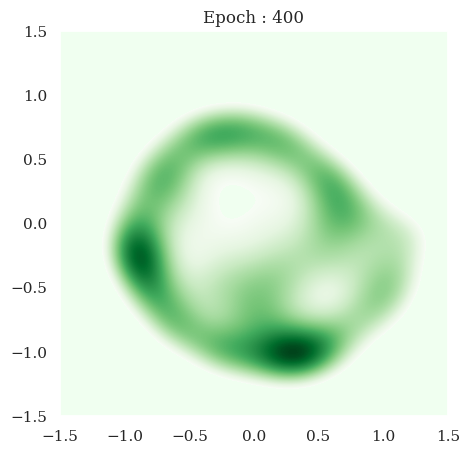
\includegraphics[scale = 0.2]{fig2-1.png}
        }
        \subfigure[]{
            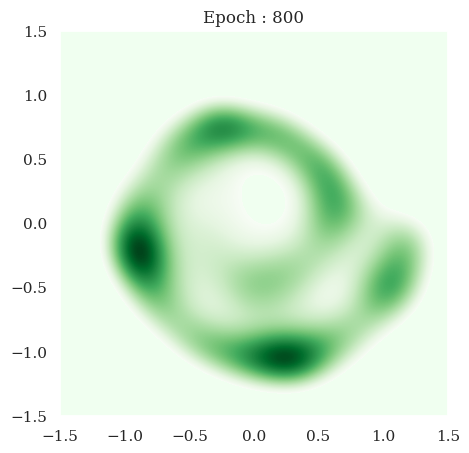
\includegraphics[scale = 0.2]{fig2-2.png}
        }
        \subfigure[]{
            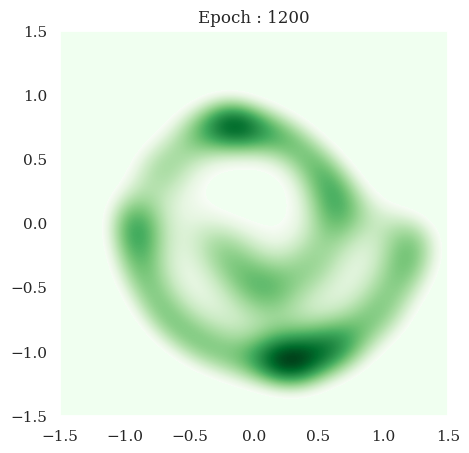
\includegraphics[scale = 0.2]{fig2-3.png}
        }
        \subfigure[]{
            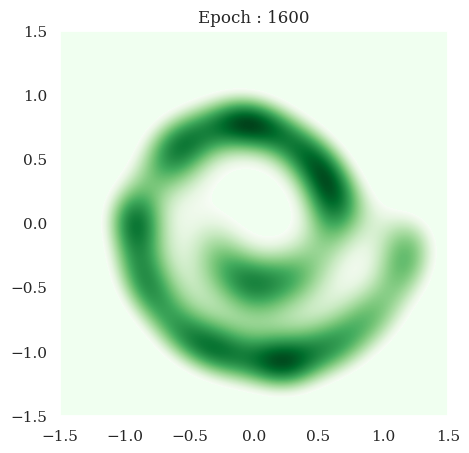
\includegraphics[scale = 0.2]{fig2-4.png}
        }
        \subfigure[]{
            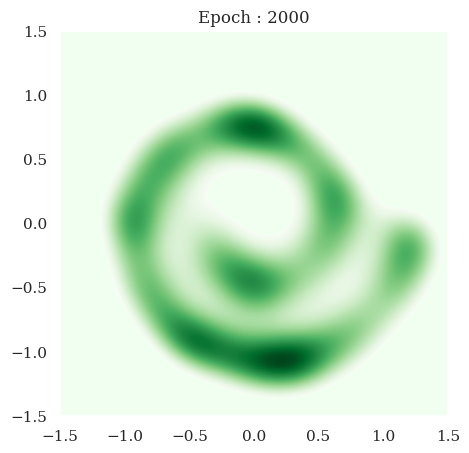
\includegraphics[scale = 0.2]{fig2-5.png}
        }
        \caption{(a) The reconstruction of Swiss roll data via VAE at 400 epochs.(b) The reconstruction of Swiss roll data via VAE at 800 epochs. (c) The reconstruction of Swiss roll data via VAE at 1200 epochs. (d) The reconstruction of Swiss roll data via VAE at 1600 epochs. (e) The reconstruction of Swiss roll data via VAE at 2000 epochs.}
        \label{fig2}
    \end{center}
\end{figure}
\begin{figure}[!h]
    \begin{center}
        \subfigure[]{
            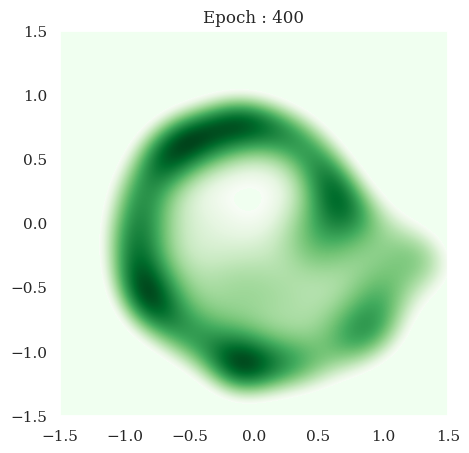
\includegraphics[scale = 0.2]{fig3-1.png}
        }
        \subfigure[]{
            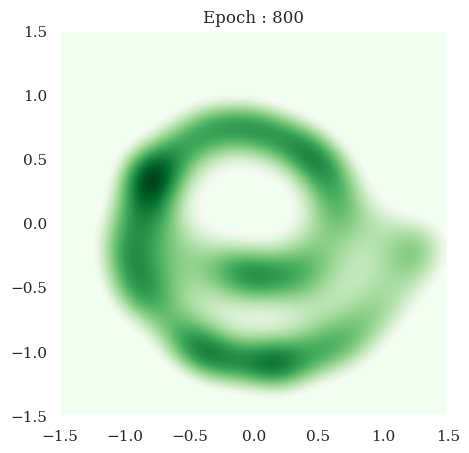
\includegraphics[scale = 0.2]{fig3-2.png}
        }
        \subfigure[]{
            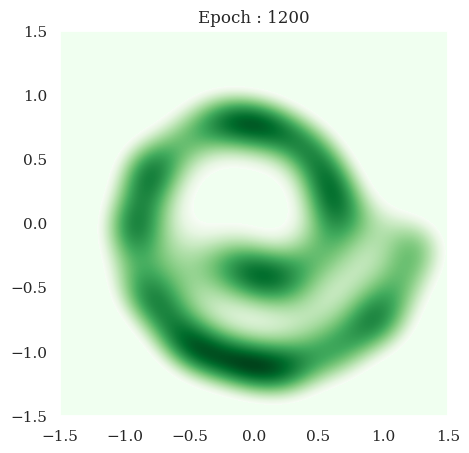
\includegraphics[scale = 0.2]{fig3-3.png}
        }
        \subfigure[]{
            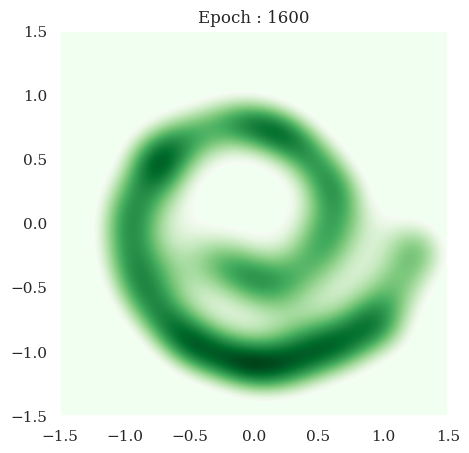
\includegraphics[scale = 0.2]{fig3-4.png}
        }
        \subfigure[]{
            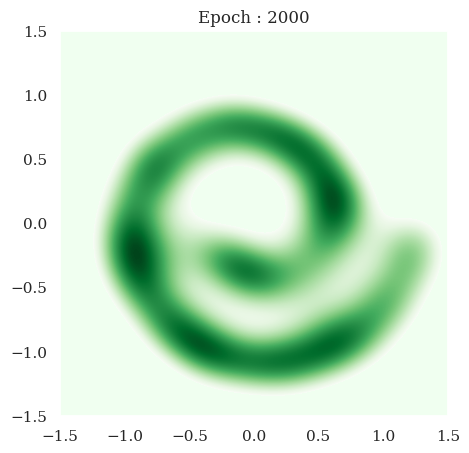
\includegraphics[scale = 0.2]{fig3-5.png}
        }
        \caption{(a) The reconstruction of Swiss roll data via GAN at 400 epochs.(b) The reconstruction of Swiss roll data via GAN at 800 epochs. (c) The reconstruction of Swiss roll data via GAN at 1200 epochs. (d) The reconstruction of Swiss roll data via GAN at 1600 epochs. (e) The reconstruction of Swiss roll data via GAN at 2000 epochs.}
        \label{fig3}
    \end{center}
\end{figure}


\end{document}